\documentclass{sprawozdanie-agh}

\usepackage[utf8]{inputenc}
\usepackage{listings}
\usepackage{babel}
\usepackage[fontsize=13pt]{scrextend}


\makeatletter

\begin{document}

\przedmiot{studio projektowe I}
\tytul{Trajektorie dzienne w technologii blockchain}
\podtytul{Przechowywanie trajektorie przemieszczeń przy użyciu technologii blockchain }
\kierunek{informatyka}
\autor{Dmytro Kuzmin\qquad Vyacheslav Trushkov}
\data{Kraków, 21 kwietnia 2021}

\stronatytulowa{}
\tableofcontents 
\newpage
\section{Wprowadzenie}
Przedstawiamy dokumentację dotyczącą projektu realizowanego w ramach przedmiotu Studio Projektowe I. Projekt polega na zrobieniu systemu do przechowywania trajektorii przy użyciu technologii blockchain.

\section{Motywacja}
Załóżmy że mamy flotę samochodów zajmującą się dostawą towarów. Chcemy mieć podgląd do przebytej drogi każdego samochodu. Dlatego możemy stworzyć rozproszoną sieć która przechowuję historię przebytych tras każdego z samochodów należących do naszej floty. Dane będą przechowywane bez możliwości edycji co zapewni nam pewność że otrzymujemy dane wiarygodne. Wyżej opisane własności możemy otrzymać używając technologii blockchain. 

\section{Wprowadzenie teoretyczne}
\subsection{Blockchain}
Do tworzenia rozproszonej bazy danych używamy blockchain. \\
Blockchain trajektorii przemieszczeń to jest zdecentralizowany rejestr łączonych do bloków transakcji, zawierających w sobie trasę i jej autora, funkcjonujący jako rosnąca lista jednokierunkowa. To jest kluczowy sposób strukturyzacji danych, odróżniający Blockchain od zwykłej bazy danych. Blockchain gromadzi informacje w grupach, zwanych również blokami, które przechowują zestawy informacji. Jeden blok w Blockchain trajektorii przemieszczeń jest tworzony średnio raz na 8 godzin. Bloki nie mają określonej pojemności, więc wszystkie otrzymane transakcję są łączone blokiem z poprzednim raz na 8 godzin, tworząc łańcuch danych znany jako „łańcuch bloków”.Wszystkie nowe informacje wynikające ze świeżo dodanego bloku są kompilowane do nowo utworzonego bloku, który po wypełnieniu zostanie również dodany do łańcucha. System ten z natury tworzy również nieodwracalny harmonogram danych, gdy jest wdrażany w sposób zdecentralizowany.
\begin{figure}[htbp]
    \centerline{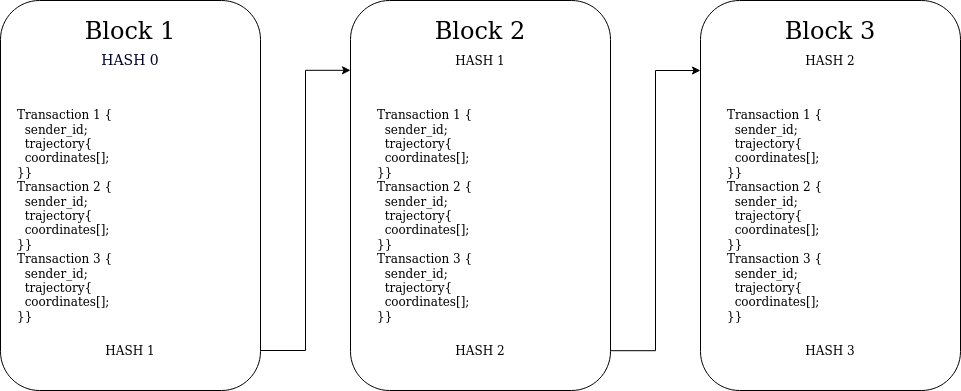
\includegraphics[width=480px, height=180px]{blockchain.png}}
    \caption{Rysunek pokazuje strukturę blockchain'u trajektorii przemieszczeń}
    \label{fig}
\end{figure}

\subsection{Budowa blockchain'u}
Blockchain składa się z bloków które z kolei składają się z transakcji. 
\subsubsection{Transakcje}
Transakcje są podstawową jednostką informacji w naszym systemie. \\
Transakcja zawiera w sobie takie pola:
   \begin{itemize}
     \item ID samochodu
     \item Długość trasy
     \item Lista współrzędnych trasy 
   \end{itemize}
Kiedy samochód rozpoczyna trasę to transakcja zostaję stworzona lokalnie i co jakiś czas zostaję aktualizowana. Transakcja zostaję zakończona wraz z zakończeniem trasy. Co 8 godzin transakcji ze wszystkich samochodów zostają przesłane do głównego komputera na którym tworzymy Block.
\subsubsection{Block}
Block będzie tworzony każde 8 godzin (zakładamy że zmiana kierowcy będzie 8 godzin). Blok zawiera w sobie transakcji i hash'e poprzednich bloków. \\
Block zawiera w sobie takie pola:
   \begin{itemize}
     \item Hash poprzedniego bloku 
     \item Data utworzenia
     \item Hash transakcji za ostatnią zmianę
   \end{itemize}

\begin{figure}[htbp]
    \centerline{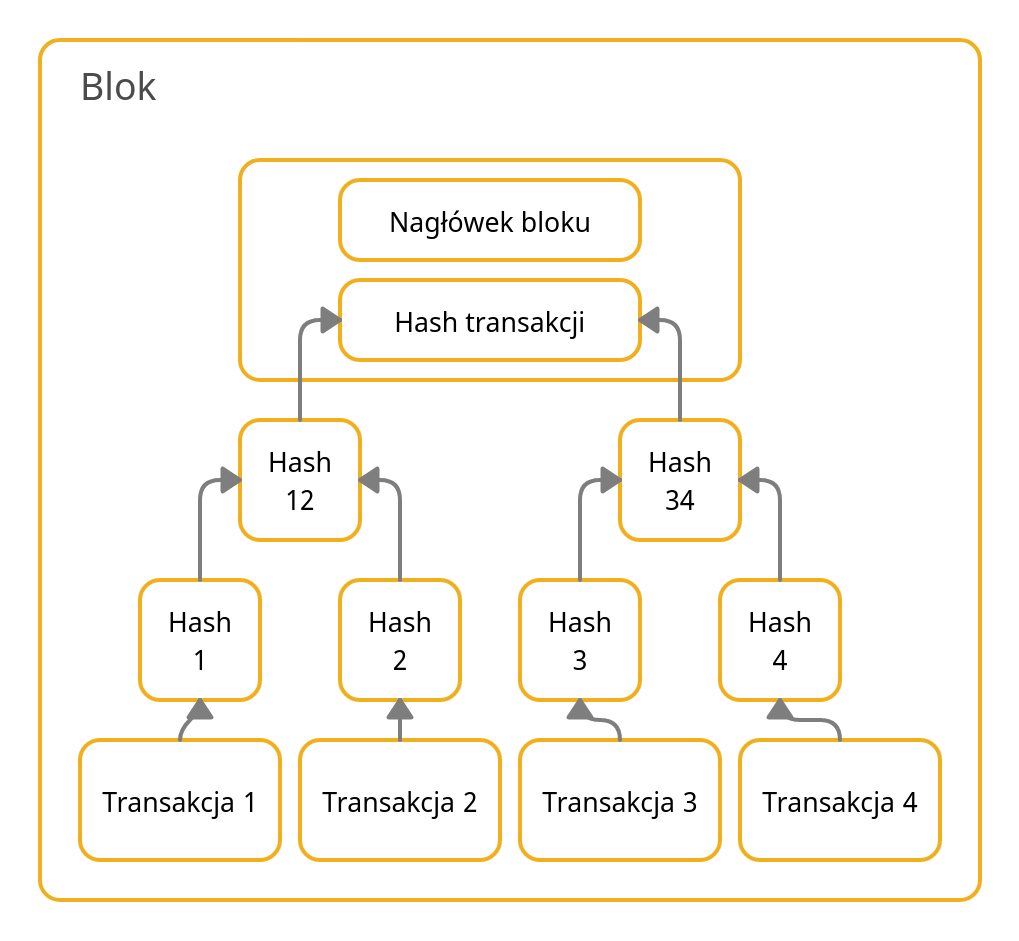
\includegraphics[width=300px, height=250px]{block.png}}
    \caption{Rysunek pokazuje strukturę blocku}
    \label{fig}
\end{figure}
\newpage
\subsection{Bezpieczeństwo}
Jedną z głównych zalet blockchainu jest niezmienność danych. Jest to powodowane tym że gdy chcemy zmienić jakiś blok to musimy wprowadzić zmianę do wszystkich kopij naszego blockchainu co w praktyce staję się praktycznie nierealnie. \\ \\
Z racji na to że każdy następny blok powstaję z hash'ów poprzednich bloków to nie możemy zmieniać bloków. Gdyż zostanie wprowadzona zmiana do już istniejącego bloku to hash zmienionego bloku już się nie będzie zgadzał z tym hashem który jest zapisany w następnym bloku, i możemy powiedzieć że obcinamy relację pomiędzy blokami. 
\begin{figure}[htbp]
    \centerline{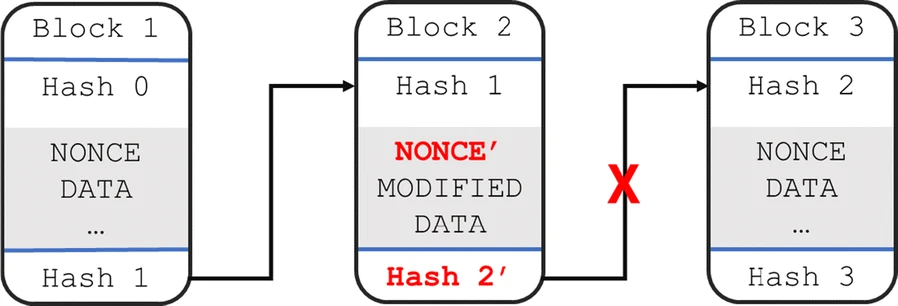
\includegraphics[width=300px, height=100px]{invalid_block.png}}
    \caption{Rysunek pokazuje blockchain z modyfikowanymi danymi w block 2}
    \label{fig}
\end{figure}

\newpage
\subsection{Uzasadnienie wyboru}
\subsubsection{Jeden blok zawiera wszystkie transakcji}
Koncepcja polega na tym że nasz blockchain tworzy swojego rodzaju dziennik. W danym dzienniku jedna strona reprezentuje jedną zmianie, a strona z kolei reprezentuje jeden blok. \\ 
Przechowując wszystkie trajektorie dzienne, a nie każdą trajektorie w bloku. Unikamy sytuacji kiedy blockchain będzie się rozrastał. Na przykład może się zdarzyć że jeden kierowca będzie wskazywał początek i koniec trasy co 10m i otrzymamy duży łańcuch bloków który będzie bezsensownym.

\subsubsection{Nowy blok co 8 godzin}
Jak jest opisane powyżej, chcemy przechowywać jedną zmianę w blockchainu, z tego wynika że potrzebujemy stałego czasu zapisywania do bloku, żeby ujednolicić wszystkie zapisy do blockchainu.
\subsubsection{Algorytm Konsensusu: Proof Of Work}
Najważniejszą celą metod osiągania konsensusu jest zapewnianie bezpieczeństwa sieci za rachunek tworzenia 'kosztu' każdego utworzonego bloku. Wiedząc że hash każdego z bloków bazuje się na hashu bloku poprzedniego, widzimy, że jeżeli jakaś informacja w historii bloków została zmieniona to wtedy trzeba byłoby wykonać pracę mainerów (w naszym przypadku komputera głównego) od zmodyfikowanego bloku do ostatniego. Czyli tworzymy sytuację, kiedy straty czasu i kosztów na zmianę historii blockchain'u są za duże, czym zapewniamy niezmienność historii.\\
Do wyboru mieliśmy zasadniczo dwa algorytmy konsensusu:
\begin{itemize}
    \item \textbf{Proof of Space} - Jest formą kryptograficznego potwierdzenia, w którym jedna strona udowadnia innym, że pewna ilość przestrzeni została poświęcona na jakiś cel.
    \item \textbf{Proof of Work} - Jest formą kryptograficznego potwierdzenia, w którym jedna strona udowadnia innym, że pewien wysiłek obliczeniowy został poświęcony na jakiś cel.
\end{itemize}
    Podstawową różnicą wad i zalet pomiędzy pierwszym a drugim jest wysokie zużycie prądu algorytmem Proof od Work, wtedy kiedy Proof of Space jest bardziej ekologiczny i ma dużo niższe zużycie. Z drugiej strony Proof of Work jest prostszy w implementacji i przy niskiej mocy sieci zwiększa koszt bloku z upływem czasu, gdyż Proof of Space potrzebuje dodatkowej kontroli w postaci Proof of Elapsed Time. Licząć że będziemy mieć sieć zamkniętą o niskiej mocy, stosunkowe zużycie prądu będzie nieistotne, więc w naszym przypadku decydujemy, że Proof of Time będzie lepszy.
\newpage

\subsection{Nonce o stałej złożoności}
        Przewidujemy, że sieć będziemy zamknięta i będzie posiadała stałą moc obliczeniową, więc ustalając jeden raz złożoność nie będziemy mieli potrzeby ją zmieniać.


\section{Opis systemu} 
\subsection{Ogólny opis}
System będzie się składał z \textbf{komputera głównego}, który będzie tworzył \textbf{blockchain}, z \textbf{floty samochodów} które przesyłają swoje trasy do głównego komputera.
\begin{figure}[htbp]
    \centerline{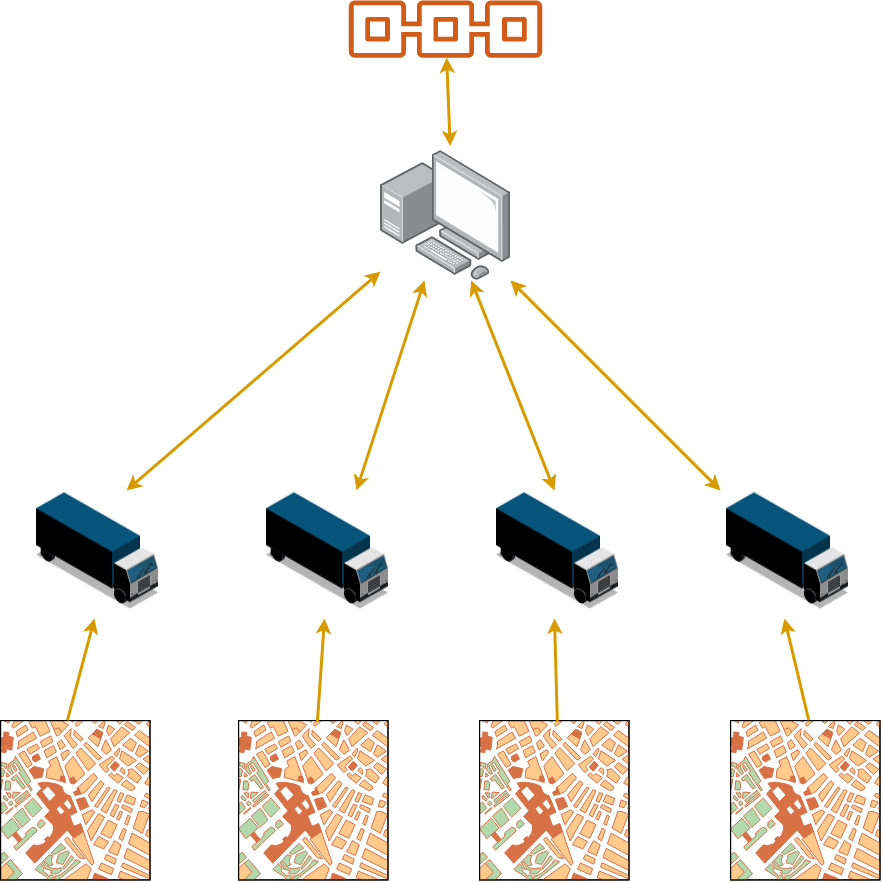
\includegraphics[width=300px, height=300px]{system_sheme.png}}
    \caption{Rysunek pokazuję ogólny schemat systemu}
    \label{fig}
\end{figure}
Każdy samochód po przebyciu trasy będzie zapisywała to lokalnie na urządzeniach wbudowanych do samochodu. Każdy samochód będzie miał swoje ID co pozwoli na szybką identyfikację który samochód jaką trasę przebył. Po rozpoczęciu trasy urządzenie które jest podłączone do GPS będzie próbkować współrzędne z ustawionym okresem. Lista współrzędnych która jest sama w sobie strukturą losową formuję transakcję. \\  
Jedną transakcja jest to jedna trasa. Zapisujemy do transakcji ID samochodu dlatego żeby było możliwie przydzielić samochód do trasy. Trasę zapisujemy dlatego że interesuję nas historia przejazdów danego samochodu. Długość trasy zapisujemy dlatego żeby nie tracić dokładności przy wyliczaniu długości z współrzędnych. 
\newpage
\subsection{Algorytm}
\begin{figure}[htbp]
    \centerline{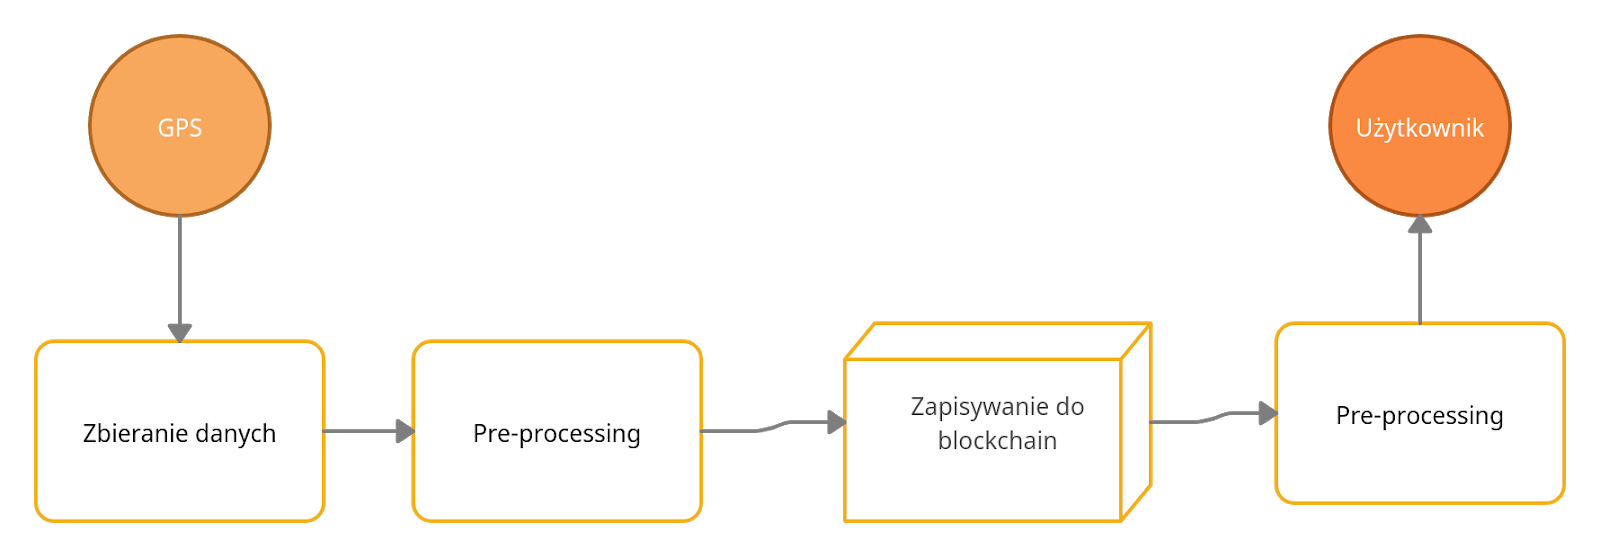
\includegraphics[width=400px,height=135px]{algo_blockchain.png}}
    \caption{Rysunek pokazuję ogólny schemat algorytmu}
    \label{fig}
\end{figure}
Algorytm składa się z czterech punktów.

\begin{itemize}
  \item \textbf{Zbieranie danych} polega na próbkowaniu danych z GPS.
  \item \textbf{Pre-processing} polega na tworzeniu transakcji która zostanie zapisana do blockchain.
  \item \textbf{Zapis do blockchain}, na tym etapie zostaną zebrane wszystkie transakcję z ostatniej zmiany i z tych transakcji zostanie utworzony nowy block. 
  \item \textbf{Pre-processing} dany pre-processing służy do odczytania danych z blockchain i przedstawieniu ich użytkowniku.
\end{itemize}

\section{Implementacja}
\subsection{Opis technologii}
\begin{itemize}
    \item Język programowania: \textbf{Python}\\
    \begin{itemize}
    \item Python wspiera różne paradygmaty programowania - pozwala zastosować programowanie obiektowe żeby
    implementować każdą składową łańcuchu bloków osobno oraz programowanie funkcyjne żeby w łatwy i czytelny sposób
    zarządzać dużą ilością uporządkowanych danych.
    \item Automatyczne zarządzanie pamięcią w Pythonie za pomocą Garbage Collector wezmę na siebie odpowiedzialność za de-alokację niepotrzebnej pamięci, za rachunek czego zwiększa się poziom bezpieczeństwa systemu.
    \item Wielka ilość wspieranych platform.
    \end{itemize}

    \item Biblioteki: \textbf{Numpy, json}
    \begin{itemize}
    \item Wiadomo że Python ma stosunkowo niską wydajność. Ten problem rozwiązujemy za pomocą biblioteki Numpy,
    która jest zaimplementowana w języku C. Takie rozwiązanie pozwoli pozwoli zapewnić wysoką szybkość obliczeń na
    na tablicach danych.
    \item JSON będzie wykorzystany żeby przedstawić dane w wygodnej postaci dla funkcji hashującej SHA256.
    \end{itemize}
    
    \item API: \textbf{Mapbox}
        \begin{itemize}
            \item Mapbox zostanie wykorzystany do wizualizacji otrzymanych tras
        \end{itemize}
        
    \item Algorytm Kosensusu: \textbf{Proof Of Work} 
    \begin{itemize}
            \item w technologii blockchain to jest technika osiągania porozumienia w kwestii dodawania nowych bloków.
            Pozwala komputeru udowodnić że na dodanie nowego bloku został poświęcony pewny wysiłek obliczeniowy. W naszym przypadku to będzie znajdowanie liczby Nonce o \textbf{stałej} złożoności.
    \end{itemize}
    
\end{itemize}

\newpage
\subsection{Diagramy klas}
    \begin{figure}[htbp]
        \centerline{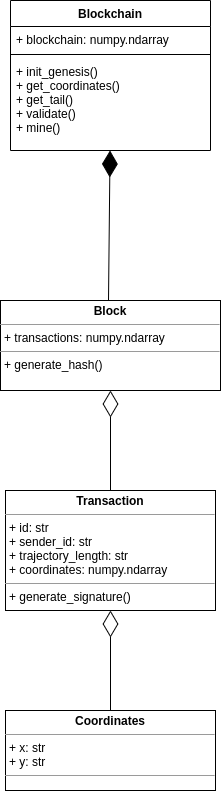
\includegraphics[width=140px,height=500px]{Blockchain.png}}
        \caption{Rysunek pokazuję klasy programu oraz najważniejsze pola i funkcję}
        \label{fig}
    \end{figure}


\newpage
\subsection{Endpoints}

\begin{itemize}
    \item \textbackslash  - genesis
    \item \textbackslash nodes\textbackslash register - dodać nową nodę
    \item \textbackslash nodes\textbackslash resolve - znaleźć konsensus
    \item \textbackslash transactions\textbackslash new - dodać nową transakcję
    \item \textbackslash mine - zapisać blok
    \item \textbackslash chain - otrzymać cały blockchain
    
\end{itemize}




\end{document}